\section{Planificaci\'on del Proyecto}\label{sec:planificacion}

La red actual que consta de conexiones físicas de fibra oscura monomodo G.652.D no tiene dinamismo y no se le esta sacando provecho. Es por esto que se pretende establecer una red inteligente basada en DWDM. La fibra G.652.D posee unas tasas de corte de $0.01$ y $0.05 [\frac{\text{cortes}/\text{año}}{\text{km}}]$ en zona rural y zona metropolitana respectivamente. Dados estos parámetros se desea implementar una red interconectada que garantice cierto estándar de disponibilidad ($\geq 99.999\%$) de conectividad entre todos sus puntos para una ventana de reparación de $8$ horas.

El diseño de los caminos de la red se realizó utilizando el algoritmo descrito en \ref{sec:algoritmo_conex}. Para entender como funciona el algoritmo hay que definir algunos conceptos preliminares. Existen dos tipos de conexiones: físicas directas y virtuales. Las conexiones físicas corresponden a las fibras oscuras que conectan cada par de datacenter (ver Figura \ref{fig:diagrama_red}. Vale la pena notar que este tipo de conexiones no existe entre todos los datacenter. Distinto es el caso de las conexiones virtuales las cuales pueden ser directas o indirectas. Por ejemplo, una conexión virtual se puede establecer entre los datacenter LONG y CNT a traves de una conexión física directa o entre los datacenter CDV y NNA a través de CNT, usando las conexiones físicas entre CDV-CNT y CNT-NNA.

Como cada par de datacenters debe tener una conexión que cumpla con estándares preestablecidos de disponibilidad, se requiere que existan caminos suficientes para que la probabilidad de indisponibilidad (probabilidad de corte acumulado) sea menor al umbral fijado. Los resultados del algoritmo se muestran en la Figura \ref{fig:caminos}.\\

\begin{table}[!hbt]
\begin{center}
\begin{tabular}{||l | c | c | c | c | c | c||}
\hline
\hline
 & \textbf{CNT} & \textbf{CDV} & \textbf{LONG} & \textbf{SMH} & \textbf{NNA} & \textbf{LCD}  \\
\hline
\textbf{CNT} & ... & (1,2),(1,4,2) & (1,3),(1,2,3) & (1,4),(1,6,4) & (1,5),(1,6,5) & (1,6),(1,5,6)\\
\hline
\textbf{CDV} &  & ... & (2,3),(2,1,3) & (2,4),(2,1,4) & (2,1,5),(2,4,6,5) & (2,4,6),(2,1,6)\\
\hline
\textbf{LONG} &  &  & ... & (3,2,4),(3,1,4) & (3,1,5),(3,2,4,6,5) & (3,1,6),(3,2,4,6)\\
\hline
\textbf{SMH} &  &  &  & ... & (4,1,5),(4,6,5) & (4,6),(4,1,6)\\
\hline
\textbf{NNA} & & & & & ... & (5,6),(5,1,6)\\
\hline
\textbf{LCD} & & & & & & ... \\
\hline
\end{tabular}
  \caption[Caminos calculados por algoritmo de disponibilidad]{Caminos que aseguran el estándar de SLA del 0.01\% de indisponibilidad por 2 días. Calculados con algoritmo de la sección \ref{sec:algoritmo_conex}}.
  \label{fig:caminos}
\end{center}
\end{table}

%\begin{figure}[H]
%  \centering
%  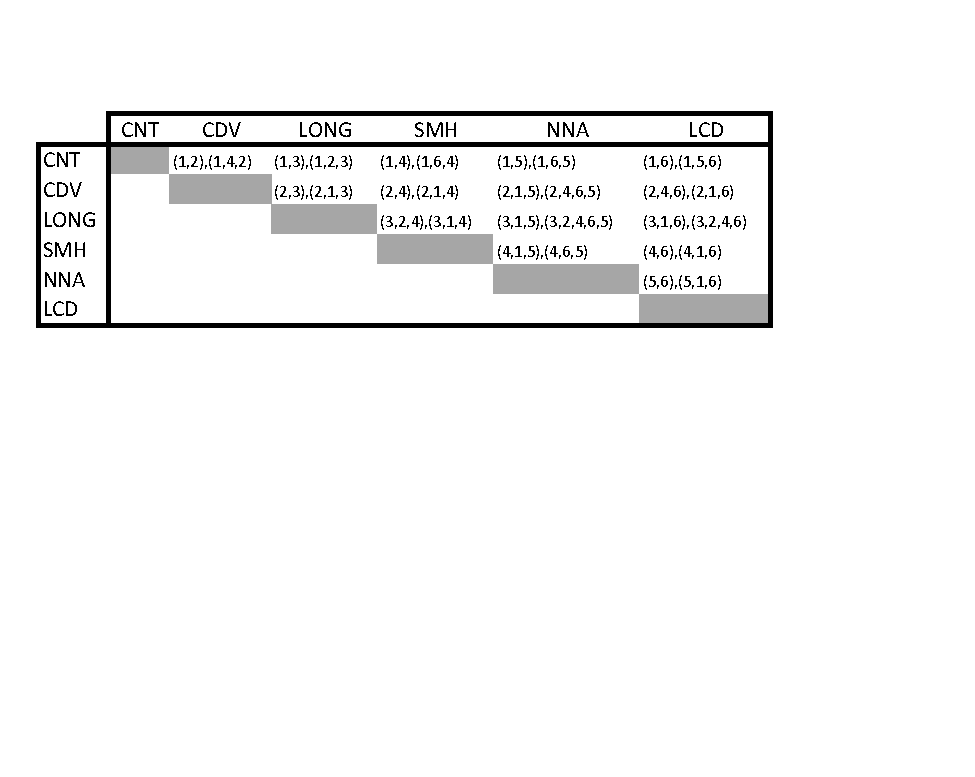
\includegraphics[width=13cm]{Imagenes/caminos.pdf}
%  \caption[Caminos calculados por algoritmo de disponibilidad]{Caminos que aseguran el estándar de SLA del 0.01\% de indisponibilidad por 2 días. Calculados con algoritmo de la sección \ref{sec:algoritmo_conex}}.
%  \label{fig:caminos}
%\end{figure}

Considerando la cantidad de servicios requeridos en el proyecto (ver Tablas \ref{tab:10ge} y \ref{tab:FC4G}), se puede calcular la cantidad de canales disponibles que deben existir en cada datancenter para cumplir con la demanda propuesta con los estándares de cálidad proporcionados. Los resultados se muestran en la figura \ref{fig:puertas} para los servicios 10GE y Fiber Channel 4G. Si se considera que por cada servicio 10GE y por cada 2 Fiber Channel 4G se debe utilizar 1 de los 80 $\lambda$ que se pueden montar en la fibra G.652.D, la cantidad de pares de fibras ópticas (Tx y Rx) necesarias en cada datacenter se especifican en la figura \ref{fig:pelos}.

\begin{table}[!hbt]
\begin{center}
\begin{tabular}{||l | c  c  c  c  c  c||}
\hline
\hline
 \textbf{\textit{10GE}}& \textbf{CNT} & \textbf{CDV} & \textbf{LONG} & \textbf{SMH} & \textbf{NNA} & \textbf{LCD}  \\
\hline
\textbf{CNT} & ... & 120 & 50 & 24 & 24 & 52\\
\hline
\textbf{CDV} &  & ... & 50 & 28 & 0 & 0\\
\hline
\textbf{LONG} &  &  & ... & 0 & 0 & 0\\
\hline
\textbf{SMH} &  &  &  & ... & 0 & 28\\
\hline
\textbf{NNA} & & & & & ... & 24\\
\hline
\textbf{LCD} & & & & & & ... \\
\hline
\end{tabular}
\end{center}
\end{table}

\begin{table}[!hbt]
\begin{center}
\begin{tabular}{||l | c  c  c  c  c  c||}
\hline
\hline
 \textbf{\textit{FC4G}}& \textbf{CNT} & \textbf{CDV} & \textbf{LONG} & \textbf{SMH} & \textbf{NNA} & \textbf{LCD}  \\
\hline
\textbf{CNT} & ... & 180 & 100 & 24 & 24 & 42\\
\hline
\textbf{CDV} &  & ... & 100 & 28 & 0 & 0\\
\hline
\textbf{LONG} &  &  & ... & 0 & 0 & 0\\
\hline
\textbf{SMH} &  &  &  & ... & 0 & 28\\
\hline
\textbf{NNA} & & & & & ... & 24\\
\hline
\textbf{LCD} & & & & & & ... \\
\hline
\end{tabular}
\caption[Puertas de cada DataCenter]{Puertas necesarias en cada datacenter. Algunas son usadas como nodo de paso, y otras son punto de inicio/final de la comunicación.}
  \label{fig:puertas}
\end{center}
\end{table}


%\begin{figure}[H]
%  \centering
%  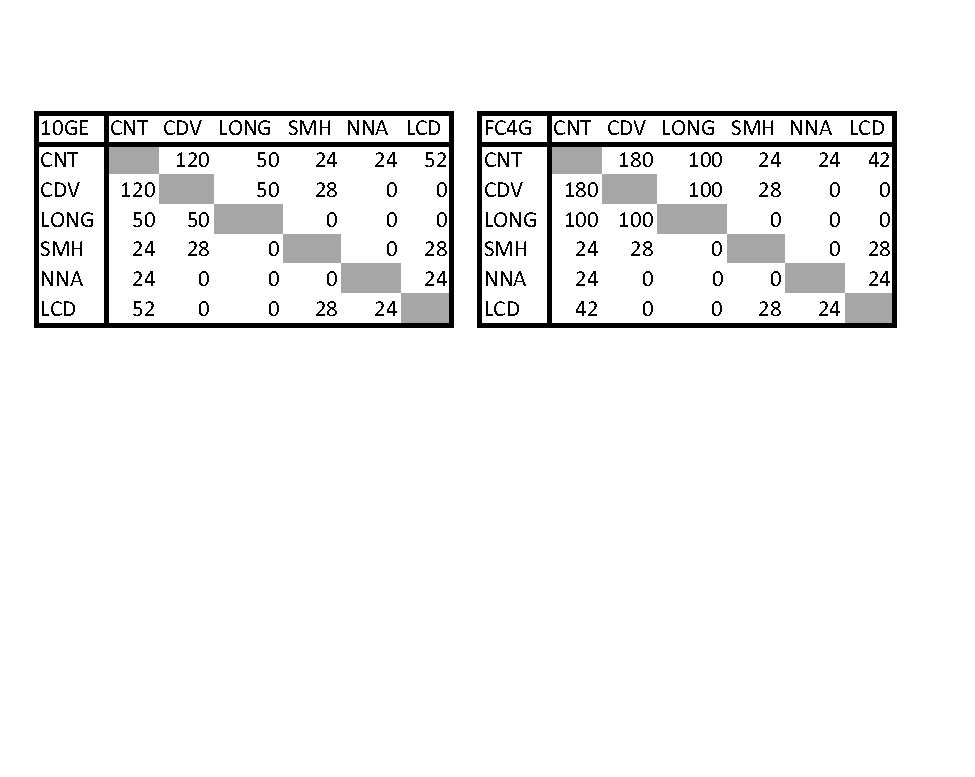
\includegraphics[width=13cm]{Imagenes/puertas.pdf}
%  \caption[Puertas de cada DataCenter]{Puertas necesarias en cada %datacenter. Algunas son usadas como nodo de paso, y otras son punto %de inicio/final de la comunicación.}
%  \label{fig:puertas}
%\end{figure}

\begin{table}[!hbt]
\begin{center}
\begin{tabular}{||l | c  c  c  c  c  c||}
\hline
\hline
 \textbf{\textit{Pelos}}& \textbf{CNT} & \textbf{CDV} & \textbf{LONG} & \textbf{SMH} & \textbf{NNA} & \textbf{LCD}  \\
\hline
\textbf{CNT} & ... & 3 & 2 & 1 & 1 & 1\\
\hline
\textbf{CDV} &  & ... & 2 & 1 & 0 & 0\\
\hline
\textbf{LONG} &  &  & ... & 0 & 0 & 0\\
\hline
\textbf{SMH} &  &  &  & ... & 0 & 1\\
\hline
\textbf{NNA} & & & & & ... & 1\\
\hline
\textbf{LCD} & & & & & & ... \\
\hline
\end{tabular}
  \caption[Fibras de cada DataCenter]{Par de pelos de Fibra Óptica necesarios en cada datacenter.}
\end{center}
\end{table}

%\begin{figure}[H]
%  \centering
%  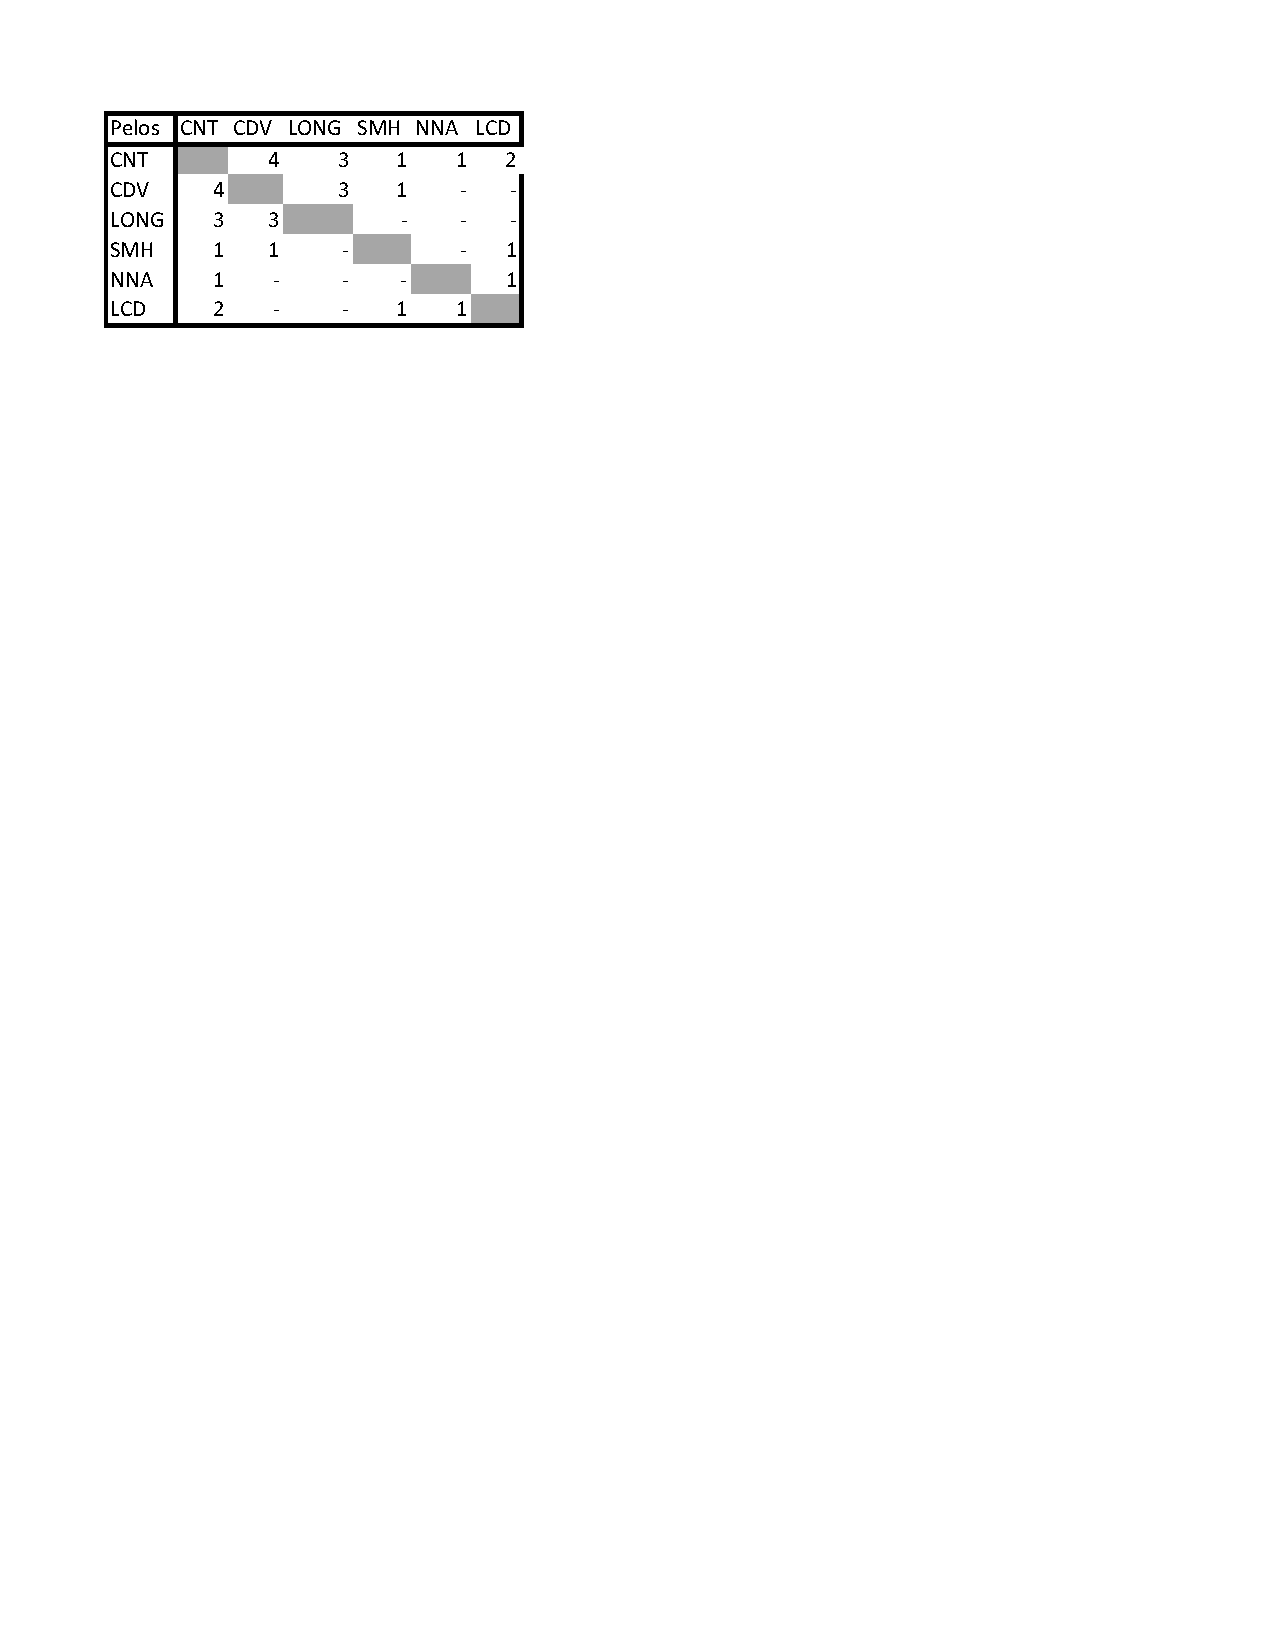
\includegraphics[width=6.5cm]{Imagenes/pelos.pdf}
%  \caption[Fibras de cada DataCenter]{Par de pelos de Fibra Óptica %necesarios en cada datacenter.}
%  \label{fig:pelos}
%\end{figure}

Teniendo en cuenta estos calculos, es posible establecer el número de equipos necesarios en cada estación. Se debe considerar primeramente una tarjeta de wavelength selective switch por cada par de fibra óptica que llega al datacenter. Además se debe considerar 1 estación local en cada DC por lo que se debe incluír un WSS adicional y un equipo de Mux/Demux de 80 canales o 2 de 40 canales debido a los requerimientos solicitados. Como la cantidad de fibras ópticas es baja será suficiente considerar un ODF para cada dirección que sale del datacenter. Esto tiene el fin de mantener un orden en los racks. Además hay que considerar los transpondedores que se utilizarán para la conversión luminica-electrica para cada servicio. El resumen de todos los equipos requeridos se muestra en la figura \ref{fig:resumen}.

\begin{table}[!hbt]
\begin{center}
\begin{tabular}{||l | c | c | c | c | c | c | c | c | c ||}
\hline
\hline
  & \textbf{ODF} & \textbf{WSS} & \textbf{MUX} & \textbf{DeMux} & \textbf{Booster} & \textbf{PreaAmp} & \textbf{Transpond.} & \textbf{Racks} & \textbf{Jumpers}  \\
\hline
\textbf{CNT} & 5 & 9 & 2 & 2 & 8 & 8 & 76 & 2 & 52\\
\hline
\textbf{CDV} & 3 & 7 & 2 & 2 & 6 & 6 & 63 & 2 & 34\\
\hline
\textbf{LONG} & 2 & 5 & 2 & 2 & 4 & 4 & 61 & 2 & 16\\
\hline
\textbf{SMH} & 3 & 4 & 2 & 2 & 3 & 3 & 33 & 2 & 12\\
\hline
\textbf{NNA} & 2 & 3 & 2 & 2 & 2 & 2 & 30 & 2 & 6\\
\hline
\textbf{LCD} & 3 & 4 & 2 & 2 & 3 & 3 & 33 & 2 & 12\\
\hline
\textbf{TOTAL} & 18 & 32 & 12 & 12 & 26 & 26 & 296 & 12 & 132\\
\hline
\end{tabular}
\caption[Total de Equipos necesarios]{Detalle de todos los equipos que se usaran en cada datancenter.}
\end{center}
\end{table}


%\begin{figure}[H]
%  \centering
%  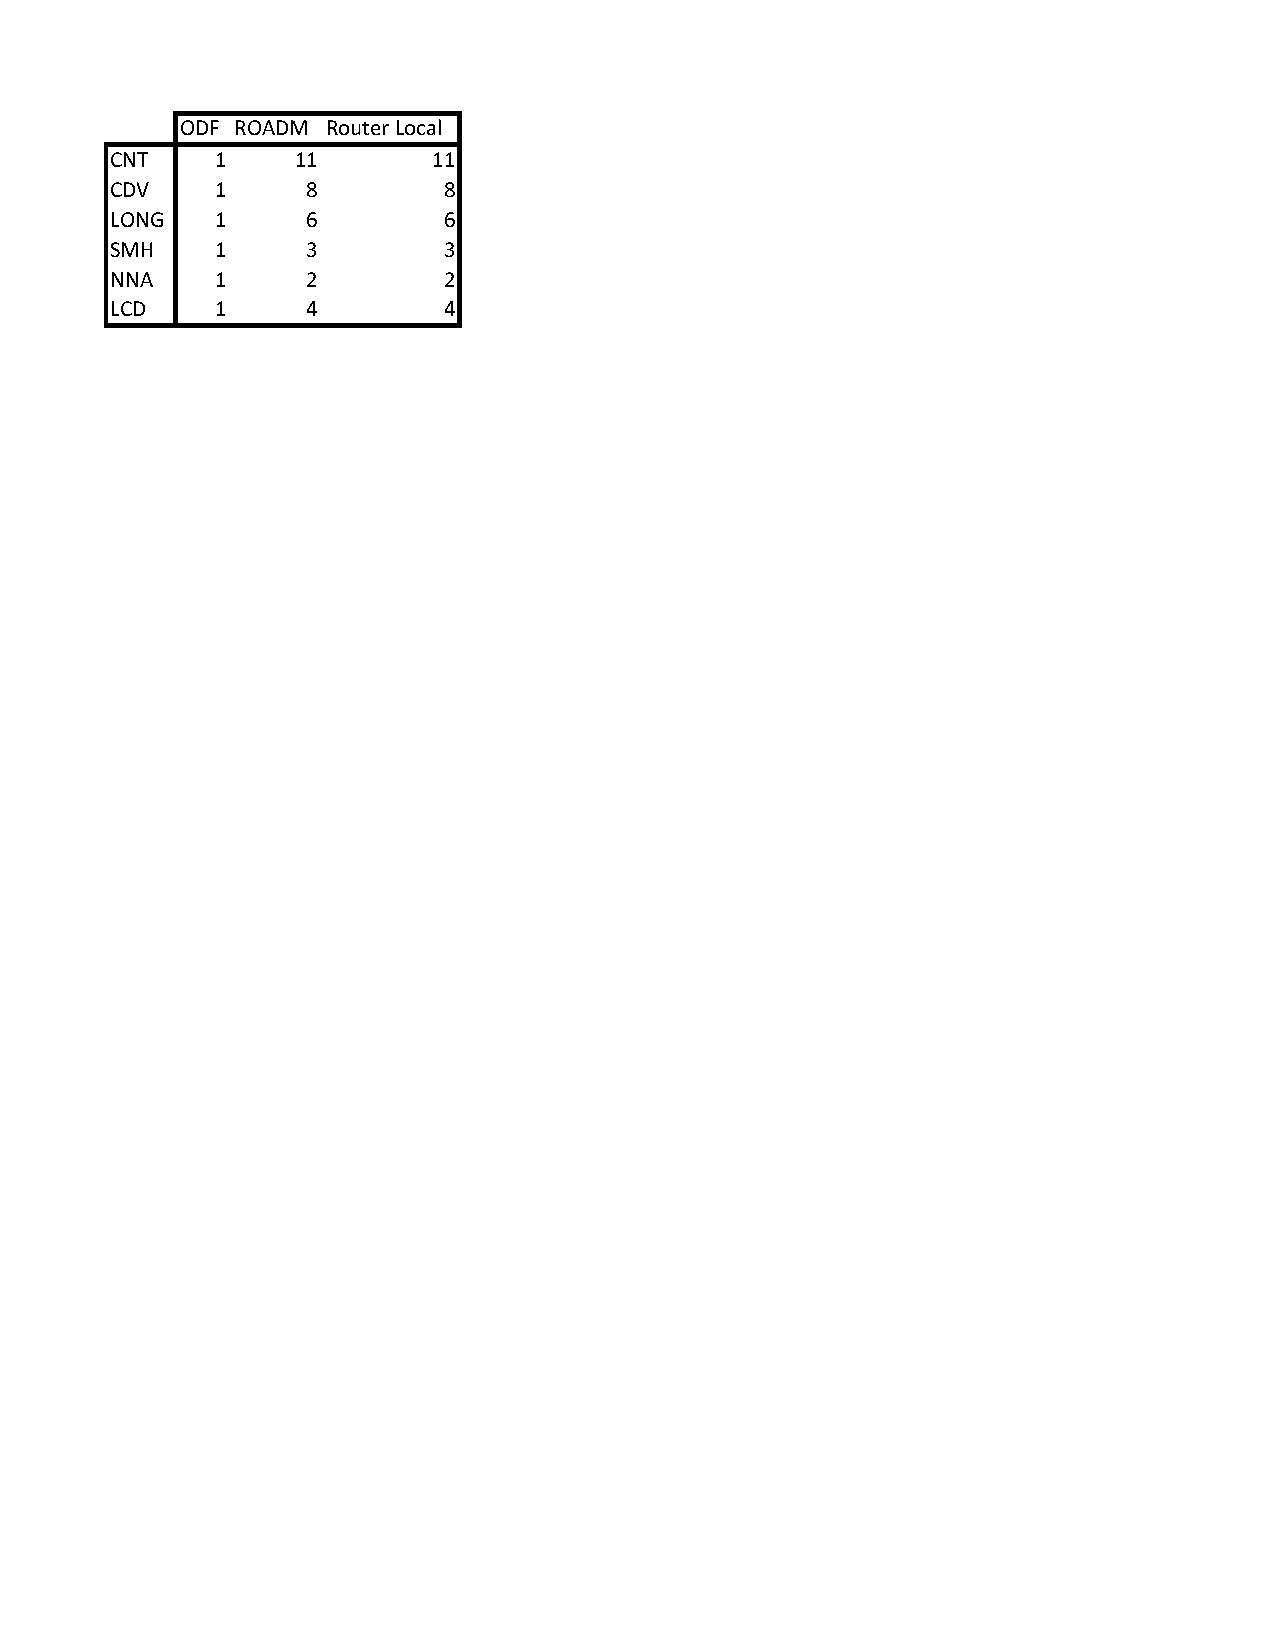
\includegraphics[width=14cm]{Imagenes/equipos.pdf}
%  \caption[Total de Equipos necesarios]{Detalle de todos los %equipos que se usaran en cada datancenter.}
%  \label{fig:resumen}
%\end{figure}

En la siguiente sección \ref{sec:ingdetalle} se especifican como deben ir conectados los equipos WSS, como deben ir los equipos puestos en los racks y un calculo de OSNR que permite estimar el nivel de ruido con el que llega la señal a cada punto.
